\documentclass[10pt]{article}\usepackage[]{graphicx}\usepackage[]{xcolor}
% maxwidth is the original width if it is less than linewidth
% otherwise use linewidth (to make sure the graphics do not exceed the margin)
\makeatletter
\def\maxwidth{ %
  \ifdim\Gin@nat@width>\linewidth
    \linewidth
  \else
    \Gin@nat@width
  \fi
}
\makeatother

\definecolor{fgcolor}{rgb}{0.345, 0.345, 0.345}
\newcommand{\hlnum}[1]{\textcolor[rgb]{0.686,0.059,0.569}{#1}}%
\newcommand{\hlsng}[1]{\textcolor[rgb]{0.192,0.494,0.8}{#1}}%
\newcommand{\hlcom}[1]{\textcolor[rgb]{0.678,0.584,0.686}{\textit{#1}}}%
\newcommand{\hlopt}[1]{\textcolor[rgb]{0,0,0}{#1}}%
\newcommand{\hldef}[1]{\textcolor[rgb]{0.345,0.345,0.345}{#1}}%
\newcommand{\hlkwa}[1]{\textcolor[rgb]{0.161,0.373,0.58}{\textbf{#1}}}%
\newcommand{\hlkwb}[1]{\textcolor[rgb]{0.69,0.353,0.396}{#1}}%
\newcommand{\hlkwc}[1]{\textcolor[rgb]{0.333,0.667,0.333}{#1}}%
\newcommand{\hlkwd}[1]{\textcolor[rgb]{0.737,0.353,0.396}{\textbf{#1}}}%
\let\hlipl\hlkwb

\usepackage{framed}
\makeatletter
\newenvironment{kframe}{%
 \def\at@end@of@kframe{}%
 \ifinner\ifhmode%
  \def\at@end@of@kframe{\end{minipage}}%
  \begin{minipage}{\columnwidth}%
 \fi\fi%
 \def\FrameCommand##1{\hskip\@totalleftmargin \hskip-\fboxsep
 \colorbox{shadecolor}{##1}\hskip-\fboxsep
     % There is no \\@totalrightmargin, so:
     \hskip-\linewidth \hskip-\@totalleftmargin \hskip\columnwidth}%
 \MakeFramed {\advance\hsize-\width
   \@totalleftmargin\z@ \linewidth\hsize
   \@setminipage}}%
 {\par\unskip\endMakeFramed%
 \at@end@of@kframe}
\makeatother

\definecolor{shadecolor}{rgb}{.97, .97, .97}
\definecolor{messagecolor}{rgb}{0, 0, 0}
\definecolor{warningcolor}{rgb}{1, 0, 1}
\definecolor{errorcolor}{rgb}{1, 0, 0}
\newenvironment{knitrout}{}{} % an empty environment to be redefined in TeX

\usepackage{alltt}
\usepackage{color}
\usepackage{graphicx} % Required for inserting
\usepackage{booktabs} % For better-quality horizontal lines
\usepackage{multirow}
\usepackage{makecell}
% \usepackage{threeparttable} % For table notes
\usepackage{array} % For table formatting
\usepackage{subcaption}
\usepackage{setspace} % For double-line spacing
\usepackage{float} 
\usepackage{tabularx}
\usepackage[round]{natbib}
\usepackage[font={small,it}]{caption}
\usepackage[utf8]{inputenc}
\usepackage{mathtools}
\usepackage{fullpage}
\usepackage{verbatim}
\usepackage{amsfonts,amssymb,amsthm}
\usepackage{url}
\usepackage[colorlinks=true,citecolor=blue]{hyperref}
% Using \doublespacing in the preamble 
% changes the text to double-line spacing
% \doublespacing

% Set page size and margins
% Replace `letterpaper' with `a4paper' for UK/EU standard size
\usepackage[a4paper,top=2cm,bottom=2cm,left=3cm,right=3cm,marginparwidth=1.75cm]{geometry}

\newcommand{\ed}[1]{\textcolor{red}{[EI: #1]}}
\newcommand{\yize}[1]{\textcolor{green}{[YH: #1]}}
\newcommand{\aaron}[1]{\textcolor{blue}{[AA: #1]}}

\bibliographystyle{apalike}
\IfFileExists{upquote.sty}{\usepackage{upquote}}{}
\begin{document}

\title{Poisson approximate likelihood compared to the particle filter}
\author{Yize Hao, Aaron A. Abkemeier and Edward L. Ionides}
\date{Draft compiled on \today}
\maketitle

\begin{abstract}
Filtering algorithms are fundamental for inference on partially observed stochastic dynamic systems, since they provide access to the likelihood function and hence enable likelihood-based or Bayesian inference.
A novel Poisson approximate likelihood (PAL) filter was introduced by \cite{wwr}.
PAL employs a Poisson approximation to conditional densities, offering a fast approximation to the likelihood function for a certain subset of partially observed Markov process models.
A central piece of evidence for PAL is the comparison in Table~1 of \cite{wwr}, which claims a large improvement for PAL over a standard particle filter algorithm.
This evidence, based on a model and data from a previous scientific study by \citet{stocks}, might suggests that researchers confronted with similar models should use PAL rather than previous particle filter methods.
Alternatively, the improvement in likelihood found by \cite{wwr} compared to \cite{stocks} might indicate a flaw in the model or numerical methods for that previous work.
We show that neither of these conclusions is valid, and the comparison of log-likelihood values made by \cite{wwr} is flawed because the PAL calculations were carried out using a dataset scaled differently from the previous study.
If PAL and the particle filter are used on this new scale, the superficial advantage of PAL largely disappears.
On simulations where the model is correctly specified, the particle filter outperforms PAL.
If a poorly fitting specification of initial value parameters is amended, the particle filter also outperforms PAL on the actual data.
\end{abstract}


% R starts here




% OvOv model is here




% Maximization Round 1 - Full rinit



% Continue: Maximization Round 2 - Full rinit



% Continue: Maximization Round 3 - Full rinit






% Maximization Round 1 - Stocks rinit



% Continue: Maximization Round 2 - Stocks rinit



% Continue: Maximization Round 3 - Stocks rinit







%%%%%%%%%% 11111111 %%%%%%%%%%%%

\section{Introduction}

This article results from an investigation of the results presented by \citet{wwr} (henceforth, WWR) in their Table~1.
WWR were given the opportunity to submit a correction, after we shared the results of our investigation with them, but they declined.
The theory developed by WWR shows that PAL has some potentially useful scaling properties, but the numerical results in Table~1 appear to show much stronger performance than a standard particle filter on an example of scientific interest but moderate size.
Our task here is to correct the error in Table~1 so that researchers considering whether to implement Poisson approximate likelihood (PAL) are appropriately informed about its benefits.

Table~1 of WWR reanalyzes the model and data of \citet{stocks} (henceforth, SBH) for which the likelihood was calculated using a particle filter.
SBH found strong evidence for the importance of overdispersion in a stochastic dynamic model for their epidemiological data.
This is significant because earlier research on population dynamics largely avoided consideration of overdispersion, perhaps because of the lack of avaialable statistical methodology to fit such models. 
The conclusions of SBH hinge on a comparison of likelihoods, and so the results of WWR discredit those conclusions by indicating that SBH based their reasoning on inaccurately computed likelihoods.
An important consequence of correcting Table~1 of WWR is that the results of SBH stand undiminished. 

SBH and WWR each fitted three different rotavirus models.
The first has equidispersion (i.e., no overdispersion) in the measurement model and the dynamic model, and is called EqEq.
The second, EqOv, includes overdispersion in only the measurement model.
The third, OvOv, includes overdispersion in both these model components.
We focus on OvOv, which WWR found to be the best fitting model. 

We show that most of the apparent advantage for PAL on the OvOv model, compared to a particle filter, arises because WWR used a different scaling of the data from SBH.
Two models for the same data can properly be compared by their likelihood, even if the models have entirely different structures.
One can make allowance for the number of estimated parameters using a quantity such as Akaike's information criterion \citep{Akaike1974ANL}.
However, if data are rescaled, a correction is required to make likelihoods comparable.
For example, if one model describes a dataset in grams and another describes it in kilograms, then the latter model will earn an increased log-likelihood of $\log(10^3)$ for each data point simply because of the change in scale.
Presenting a direct comparison of a likelihood for the data in grams with a likelihood for the data in kilograms would evidently be inappropriate.


















\begin{table}[ht] % The placement specifier can be [h!tbp]
\centering % Centers the table
\caption{AIC for the OvOv rotavirus model, computed using two filtering methods. PAL is the Poisson approximate likelihood, implemented using the code of WWR. PF is the particle filter, implemented using the code of \citet{pomppackagepaper}. The first two lines are from WWR, Table~1, and lines 3--5 are our own computations. We used 50000 particle for both PF and PAL. PF was repeated 36 times to reduce the Monte Carlo variance, but this step was not necessary for PAL.
\ed{SHOULD WE HAVE A LINE FOR PAL AT THE IF2 MLE FROM LINE 5? PERHAPS WE CAN'T READILY MAXIMIZE PAL FOR THIS MODEL (OR CAN WE?) BUT SOME SORT OF COMPARISON WOULD BE HELPFUL}
} 
\label{tab:ovovrealdata} % For referencing this table elsewhere in your text
\begin{tabular}{lllc} 
  \hline
  & Method & Result & AIC  \\
  \hline
  1. & PAL & Table~1 of WWR & 13778.08
  \\
  2. & PF & Table~1 of WWR, originally from SBH &  20134.38
  \\
  3. & PAL & Model, data and MLE from WWR &
    13814.57 
  \\
  4. & PF & Model, data and MLE from WWR &
    25785.52
  \\
  5. & PF & Data from WWR, estimated initial values &
     143875.53
  \\
  6. & PAL & Data from WWR, estimated initial values &
     15376.67
  \\
 \hline
\end{tabular}
\end{table}
 
SBH fitted their model to a dataset derived by dividing the original reported count data by an estimated reporting rate, to put their data on the scale of the actual number of cases in the population, whereas WWR fitted directly to the report data.
The reporting rate used by SBH varied over time, but was generally around $7\%$.
On approximately 1200 data points, this corresponds to a discrepancy of around $-1200\log(0.07) \approx 3200$ log-likelihood units, largely explaining the difference reported in Table~1 and interpreted by WWR as evidence supporting PAL.
The comparison can be corrected either by applying the method of SBH to the data of WWR or vice versa.
Since the method of SBH is applicable to a more general class of models, and supported by published software, it was convenient to apply the SBH method to the model and data of WWR.
The large discrepancy in log-likelihood disappears at this point by recomputing the likelihood of the model using PAL and particle filter separately (see Table~\ref{tab:ovovrealdata}).
This re-analysis does, however, show a discrepancy between two methods.
We continued our investigation to establish the cause of this.
We discovered that the initial conditions for the latent process in January 2001 (their time 0) were estimated by SBH. However, in WWR, they were assumed fixed and made the model fitted poorly. 


\begin{knitrout}
\definecolor{shadecolor}{rgb}{0.969, 0.969, 0.969}\color{fgcolor}\begin{figure}

{\centering \includegraphics[width=4.5in]{figure/plot2-cond-loglik-1} 

}

\caption[Conditional log-likelihoods computed using PAL (red) and PF (blue) for the rotavirus model and MLE from WWR]{Conditional log-likelihoods computed using PAL (red) and PF (blue) for the rotavirus model and MLE from WWR. We used 50000 particle for both PF and PAL. PF averaged over 36 replications to reduce the Monte Carlo variance, but this step was not necessary for PAL. The main sources of likelihood shortfall of PF are at time points $t=1, 2, 3, 11, 81, 194$, and $325-333$.}\label{fig:plot2-cond-loglik}
\end{figure}

\end{knitrout}



\begin{table}[htbp]
    \caption{Maximum likelihood estimation of parameters for the OvOv model of WWR by PAL (taken from WWR), and by iterated particle filtering implemented using {\rm \texttt{mif2}} in {\rm \texttt{pomp}} \citep{pomppackagepaper}. The initial distribution parameter \(\lambda_0 = (S_{10}, I_{10}, R_{10}, S_{20}, I_{20}, R_{20}, S_{30}, I_{30}, R_{30})\) are assumed to be fixed in \cite{wwr}. The iterated particle filtering estimates were obtained by using 3 rounds of refinement, with 100 filtering iterations, 50,000 particles, and 36 replicates in each round with the top 12 best fits in terms of likelihood chosen to be the starting value for the next round.}
    \label{tab:mlebywwr}
\begin{center}    
    \begin{tabular}{lccc}  % Left-aligned for the first column, centered for the other two columns
      \toprule
      Parameter      & PAL      & iterated filtering & iterated filtering (stocks)\\
      \midrule
      \(\beta_1\)    & 11.48     & $13.53$ & $16.53$\\
      \(\beta_2\)    & 0.25      & $0.42$ & $0.25$\\
      \(\beta_3\)    & 0.35      & $0.24$ & $0.18$\\
      \(\phi\)       & 0.14      & $0.23$   & $0.27$\\
      \(\rho\)       & 0.16      & $0.11$ & $0.13$\\
      \(\sigma^2_q\) & 0.021     & $0.052$ & $0.109$\\
      \(\sigma_\xi\) & 66.89     & $24.83$ & $24.83$\\
      \(S_{10}\)     & 3876549   & $2490623$  & $5094840$\\
      \(I_{10}\)     & 30351     & $3599$  & $2871$\\
      \(R_{10}\)     & 1315221   & $3035890$  & $124410$\\
      \(S_{20}\)     & 57139612  & $55481369$  & $57385600$\\
      \(I_{20}\)     & 871       & $222$  & $639$\\
      \(R_{20}\)     & 302852    & $42911$  & $57072$\\
      \(S_{30}\)     & 19573727  & $21155579$  & $19697600$\\
      \(I_{30}\)     & 2550      & $442$  & $174$\\
      \(R_{30}\)     & 131092    & $162190$  & $9578$\\
      \midrule
      \textbf{AIC}  & 13778.08  & $143875.53$ & $444098.92$\\
      \bottomrule
    \end{tabular}
\end{center}
\end{table}


\begin{knitrout}
\definecolor{shadecolor}{rgb}{0.969, 0.969, 0.969}\color{fgcolor}\begin{figure}

{\centering 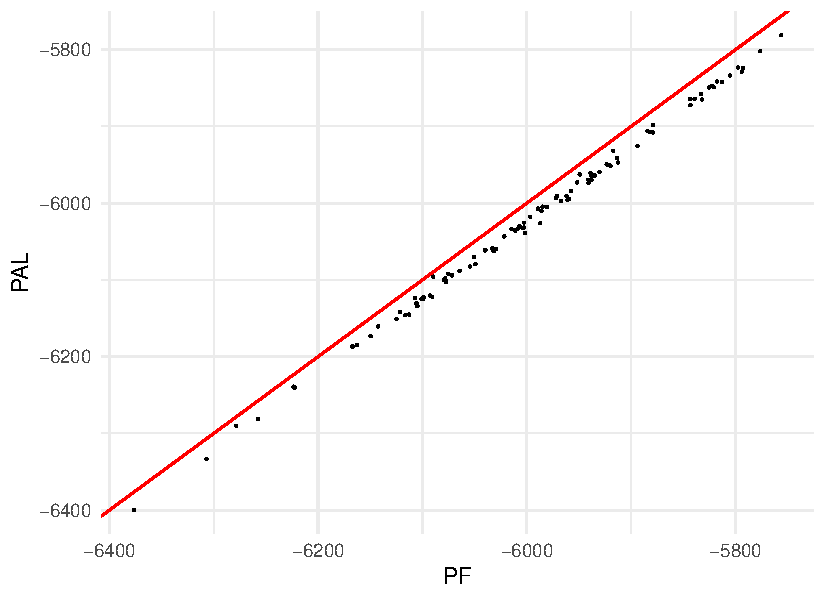
\includegraphics[width=4.5in]{figure/plot1-100-sim-compare-1} 

}

\caption[Log-likelihoods computed using two filtering methods for 100 randomly simulated datasets at the MLE of the OvOv model]{Log-likelihoods computed using two filtering methods for 100 randomly simulated datasets at the MLE of the OvOv model. Simulations with one or more zero counts were disqualified since they resulted in errors for the PAL implementation. We used 50000 particle for both PF and PAL. PF was repeated 36 times to reduce the Monte Carlo variance, but this step was not necessary for PAL. The red line corresponds to equality of the two estimates.}\label{fig:plot1-100-sim-compare}
\end{figure}

\end{knitrout}

Figure~\ref{fig:plot2-cond-loglik} indicates that the worst conditional log-likelihood values, estimated using the particle filter, arise at the start of the time series.
This could be a problem with data collection, or some subtle issue with the science of the epidemiological system, but a simple possibility is that the initial values of the latent state process might be poorly specified.
For this model, the initial values were fixed based on scientific reasoning, rather than being estimated.
If we instead estimate the initial values, we obtain the results in Table~\ref{tab:mlebywwr}. 

\ed{SINCE THE MEAN DURATION OF IMMUNITY IS 1 YR, HAVING $31\times 10^6$ in $R_{2,0}$ IMPLIES THAT ABOUT HALF OF ALL SUSCEPTIBLE INDIVIDUALS GET ROTAVIRUS EVERY YEAR ACCORDING TO THE MODEL. IS THAT THE CASE FOR THE MODEL? FOR THE DATA, THE PER-CAPITA RATE IN THIS AGE GROUP IS RATER LOW. THE SIMPLEST WAY TO AVOID THIS PROBLEM WOULD BE TO DO WHAT SBH DID (DESCRIBED IN THEIR ONLINE APPENDIX C) - EFFECTIVELY, DRAWING $X_0$ FROM THE STATIONARY DISTRIBUTION GIVEN THE MODEL. THIS HAS THE ADVANTAGE OF INCLUDING NO NEW PARAMETERS AND BEING CONSISTENT WITH SBH. WE DON'T KNOW IN ADVANCE EXACTLY HOW SUCCESSFUL IT WOULD BE...}

\section*{Discussion}

PAL provides an approximate filter, whereas the particle filter provides a Monte~Carlo estimate of an exact filter.
Possible explanations for PAL obtaining a higher log-likelihood than a particle filter include:
\begin{enumerate}
\item The particle filter could have high Monte Carlo variance. This results in negative bias in its log-likilihood estimate due to Jensen's inequality, since the particle filter provides an unbiased likelihood estimate.
\item If the model is misspecified, the approximation error in PAL could lead to a higher log-likelihood estimate than that of the actual misspecified model.
\end{enumerate}
Log-likelihood is a proper scoring rule for forecasts \cite{gneiting2}, and both the particle filter and PAL construct their log-likelihood estimates via a sequence of one-step forecasts.
Therefore, if the model is correctly specified, the approximation error in PAL can only decrease the expected log-likelihood.
We tested this on simulated data, for which the model of \cite{wwr} is correctly specified.
For this simulation study, the particle filter out-performs PAL (Figure~\ref{fig:plot1-100-sim-compare}) which supports hypothesis 2, above.
On average, the particle filter likelihood estimate is $-1027.3$ log units higher than the PAL.
Consequently, we looked for model misspecification by comparing the conditional log-likelihood estimates at each time point, as described in the Methods section.

We conclude that PAL is a potentially useful algorithm, with some favorable theoretical properties.
However, the corrected evidence does not indicate an advantage for using PAL in situations where the particle filter is effective.

%%%%%%%%% 222222222 %%%%%%%%%%

\section*{Methods}

We first replicated the model of WWR in the R package \texttt{pomp} \citep{pomppackagepaper}.
Comparing summary statistics of simulations confirms that both model versions are essentially identical, as described by \citet{hao24}.
We therefore implement PAL using the code from \citet{wwr}, comparing directly with the particle filter implemented using \texttt{pomp}.

This article has focused on likelihood evaluation, but the inferences presented also require the likelihood estimate to be maximized.
WWR used direct numerical maximization, whereas SBH used iterated filtering to maximize the particle filter likelihood estimate implemented using the \texttt{mif2} algorithm in \texttt{pomp}.
We follow the approaches adopted by these two papers.
The optimization method is not directly pertinent to the comparison of the filtering methods, so we do not discuss optimization in further detail here.
An extended description of our reanalysis of WWR is provided by \cite{hao24}.
That thesis also contains some additional results reinforcing the conclusions presented in this article.
The source code for this article is available at \url{https://github.com:ionides/pal-vs-pf} and archived at \ed{ZENODO - TODO}.

\bibliography{bib-pal}

\end{document}
